\documentclass[letterpaper]{article}
\usepackage[margin=1in]{geometry}
\usepackage[utf8]{inputenc}
\usepackage{textcomp}
\usepackage{amssymb}
\usepackage{natbib}
\usepackage{graphicx}
\usepackage{gensymb}
\usepackage{amsthm, amsmath, mathtools}
\usepackage[dvipsnames]{xcolor}
\usepackage{enumerate}
\usepackage{mdframed}
\usepackage[most]{tcolorbox}
\usepackage{csquotes}
% https://tex.stackexchange.com/questions/13506/how-to-continue-the-framed-text-box-on-multiple-pages

\tcbuselibrary{theorems}

\newcommand{\R}{\mathbb{R}}
\newcommand{\Z}{\mathbb{Z}}
\newcommand{\N}{\mathbb{N}}
\newcommand{\Q}{\mathbb{Q}}
\newcommand{\C}{\mathbb{C}}
\newcommand{\code}[1]{\texttt{#1}}
\newcommand{\mdiamond}{$\diamondsuit$}
\newcommand{\PowerSet}{\mathcal{P}}
\newcommand{\Mod}[1]{\ (\mathrm{mod}\ #1)}
\DeclareMathOperator{\lcm}{lcm}

%\newtheorem*{theorem}{Theorem}
%\newtheorem*{definition}{Definition}
%\newtheorem*{corollary}{Corollary}
%\newtheorem*{lemma}{Lemma}
\newtheorem*{proposition}{Proposition}


\newtcbtheorem[number within=section]{theorem}{Theorem}
{colback=green!5,colframe=green!35!black,fonttitle=\bfseries}{th}

\newtcbtheorem[number within=section]{definition}{Definition}
{colback=blue!5,colframe=blue!35!black,fonttitle=\bfseries}{def}

\newtcbtheorem[number within=section]{corollary}{Corollary}
{colback=yellow!5,colframe=yellow!35!black,fonttitle=\bfseries}{cor}

\newtcbtheorem[number within=section]{lemma}{Lemma}
{colback=red!5,colframe=red!35!black,fonttitle=\bfseries}{lem}

\newtcbtheorem[number within=section]{example}{Example}
{colback=white!5,colframe=white!35!black,fonttitle=\bfseries}{def}

\newtcbtheorem[number within=section]{note}{Important Note}{
        enhanced,
        sharp corners,
        attach boxed title to top left={
            xshift=-1mm,
            yshift=-5mm,
            yshifttext=-1mm
        },
        top=1.5em,
        colback=white,
        colframe=black,
        fonttitle=\bfseries,
        boxed title style={
            sharp corners,
            size=small,
            colback=red!75!black,
            colframe=red!75!black,
        } 
    }{impnote}
\usepackage[utf8]{inputenc}
\usepackage[english]{babel}
\usepackage{fancyhdr}
\usepackage{hyperref}

\pagestyle{fancy}
\fancyhf{}
\rhead{Math 187A}
\chead{Monday, January 09, 2023}
\lhead{Lecture 1}
\rfoot{\thepage}

\setlength{\parindent}{0pt}

\begin{document}
\section*{Preface}
Notes from here are adapted from \href{https://sagrawalx.github.io/assets/crypt/}{Professor Shishir Agrawal's notes for Math 187A} and modified for my own understanding.

\section{Introduction to Cryptography}
We begin with some common definitions.

\subsection{Terminology}
\begin{definition}{Cipher}{}
    A \textbf{cipher}, or cryptosystem, is a cryptographic method for confidential communication. 
\end{definition}
Generally, a cryptographic method includes algorithms for \emph{encryption} and \emph{decryption}, which are inverse processes that convert between plainly readable information called \emph{plaintext}\footnote{In cryptography, we use \emph{plaintext} and \emph{ciphertext} instead of \emph{plain text} and \emph{cipher text}.} and unintelligible information called \emph{ciphertext}.

\begin{definition}{Sender}{}
    A \textbf{sender}, often named ``Alice'' in abstract cryptographic discussions, \emph{encrypts} her plaintext into ciphertext. 
\end{definition}

\begin{definition}{Receiver}{}
    A \textbf{receiver}, often named ``Bob,'' \emph{decrypts} (or deciphers) the ciphertext back into plaintext. 
\end{definition}
Often times, Bob will use a \emph{key} to decrypt the message. This is sometimes known as a private key or decryption key.

\begin{definition}{Encoding}{}
    The (usually) preliminary step where a message is converted into a format which can then be encrypted is called \textbf{encoding}. 
\end{definition}
Note that encoded text is not secure; it is only secure after encryption. So, we can think of encoding as the pre-processing step. In other words, before we encrypt something, we might \emph{encode} the text so it's easier to encrypt. It should also be noted that if a message had to be encoded before encryption, then it will also need to be decoded after decryption. 

\begin{center}
    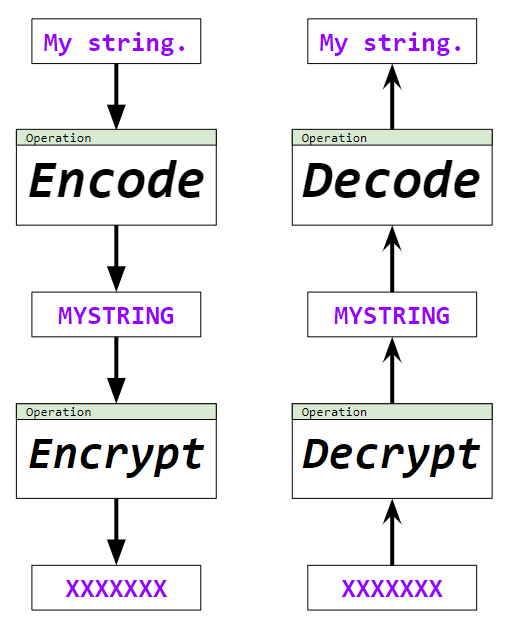
\includegraphics[scale=0.8]{../assets/encode_encrypt.png}
\end{center}

\begin{definition}{Adversary}{}
    An \textbf{adversary}, often named ``Eve,'' is one whose aim is to prevent the users of a cryptosystem from achieving their goal. 
\end{definition}
In our case here, an adversary can intercept a ciphertext. Thus, the adversary will not have Bob's decryption key at the beginning. The idea is that, even if the adversary knows what cryptosystem was used to encrypt the message, if the adversary doesn't have this decryption key, she should ideally not be able to decrypt the message. If she does manage to figure out the plaintext, she has \emph{broken} the code.

\begin{definition}{Attack Model}{}
    An \textbf{attack model} specifies what Eve is allowed to do in order to break the code. 
\end{definition}
Some common attack models includes:
\begin{itemize}
    \item Ciphertext-only attack: Eve must recover the plaintext using only the ciphertext.
    \item Known-plaintext attack: Eve may have access to some information about the plaintext (e.g., knowledge of portions of the plaintext), which can be used to recover the plaintext entirely. 
    \item Chosen-plaintext attack: Eve can request or generate ciphertexts corresponding to any plaintext message of her choosing, and she can use this information to recover the plaintext.
\end{itemize}
Classical cryptography was mostly concerned with assuring security against the first two. Modern cryptography tries to assure security against the last. 


\newpage 
\section{Classical Cryptosystems}
We begin with a definition: 
\begin{definition}{$n$-gram}{}
    An $n$-gram is a sequence of $n$ letters.
\end{definition}
For example, a 1-gram is just a single letter; a 2-gram (i.e., \emph{bigram}) is a pair of letters; and so on. Generally, we can group many classical cryptosystems into a few different encryption strategies.

\begin{center}
    \begin{tabular}{|p{1in}|p{5in}|}
        \hline
        \textbf{Strategy} & \textbf{Description} \\ 
        \hline 
        Transposition & Involves rearranging units of plaintext according to some pattern. We'll see just one example of this type of cipher: rectangular transposition. \\ 
        \hline 
        Substitution & Involves replacing units of plaintext with units of ciphertext. We can further group substitution ciphers into some subtypes: 
        \begin{center}
            \begin{tabular}{|p{1in}|p{3.5in}|}
                \hline
                \textbf{Subtype} & \textbf{Description} \\ 
                \hline
                Simple \\ Substitution & In these ciphers, single letters of plaintext are replaced by ciphertext. The substitution scheme stays the same over the course of the entire message. Some examples we'll see include:
                \begin{itemize}
                    \item Masonic cipher 
                    \item Caesar cipher 
                    \item Affine cipher 
                    \item Polybius square 
                \end{itemize}
                In essence, though, there is a 1-1 relationship between the letters of the plaintext and the ciphertext alphabets. \\
                \hline 
                Polygraphic \\ Substitution & In these ciphers, groups of letters in the plaintext are replaced by ciphertext (a group of $n$ letters is called an $n$-gram).The substitution scheme stays the same over the entire message. Some examples we'll see include: 
                \begin{itemize}
                    \item Hill cipher
                    \item Playfair cipher
                \end{itemize}
                So, in essence, polygraphic substitution is just simple substitution but with \emph{groups of letters} instead of individual letters. \\ 
                \hline 
                Polyalphabetic \\ Substitution & In these ciphers, single letters in the plaintext are replaced by ciphertext, and the substitution scheme changes over the course of the message. Some examples include: 
                \begin{itemize}
                    \item Vignere cipher 
                    \item One-time pad 
                \end{itemize} 
                \\ 
                \hline 
            \end{tabular}
        \end{center}
        In practice, however, most cryptosystems employ a combination of these strategies. \\
        \hline 
    \end{tabular}
\end{center}


















\subsection{Rectangular Tranposition}
\textbf{Rectangular tranposition}, known also as \emph{regular columnar transposition}, is a tranposition cipher. The ciphertext is obtained by \emph{permuting} the letters of the plaintext in a particular pattern. The pattern is determined by a secret \emph{keyword}. 

\bigskip 

Roughly speaking, the steps to perform rectangular transposition are as follows:
\begin{enumerate}
    \item Using the keyword, rank the letters based on alphabetical ranking. 
    \item Break up the message into groups of $n$, where $n$ is the length of the keyword.
    \item For each group, do the following: 
    \begin{itemize}
        \item Encrypting: If the $i$th letter of the keyword has rank $j$, move the $i$th letter in the group into the $j$th position.
        \item Decrypting: If the $i$th letter of the keyword has rank $j$, move the $j$th letter of each group into the $i$th position. 
    \end{itemize}
\end{enumerate}
Note that keywords with repeat letters do not work by themselves. We either need to agree not to use words with repeat letters, or remove duplicate letters from the keyword\footnote{In this course, we won't consider words with repeat letters.}.

\begin{mdframed}[]
    (Example: Encryption.) Suppose that Alice and Bob share the keyword \code{GUARD}, and that Alice wants to send the following message to Bob: 
    \begin{mdframed}
        \begin{verbatim}
Hide! The baboons are coming for you. \end{verbatim}
    \end{mdframed}

    First, we'll \textbf{encode} the message so that it's easier to encrypt. In our example, we'll remove all spaces and punctuation. 
    \begin{mdframed}
        \begin{verbatim}
HIDETHEBABOONSARECOMINGFORYOU \end{verbatim}
    \end{mdframed}
    Now that encoding is done, we still need to encrypt the message. Notice how the keyword \code{GUARD} has 5 letters; we can break the message up into 5-grams and then stack them into rows:
    \begin{mdframed}
        \begin{verbatim}
HIDET
HEBAB
OONSA
RECOM
INGFO
RYOU\end{verbatim}
    \end{mdframed}
    We then need to insert some random letters at the end of the message so every row has an equal number of letters. Let's use \code{Q}:
    \begin{mdframed}
        \begin{verbatim}
HIDET
HEBAB
OONSA
RECOM
INGFO
RYOUQ\end{verbatim}
    \end{mdframed}
    Now, we begin the \textbf{encryption} process by rearranging the letters in each row based on the alphabetical ranking of the letters of the keyword \code{GUARD}. 
    \begin{center}
        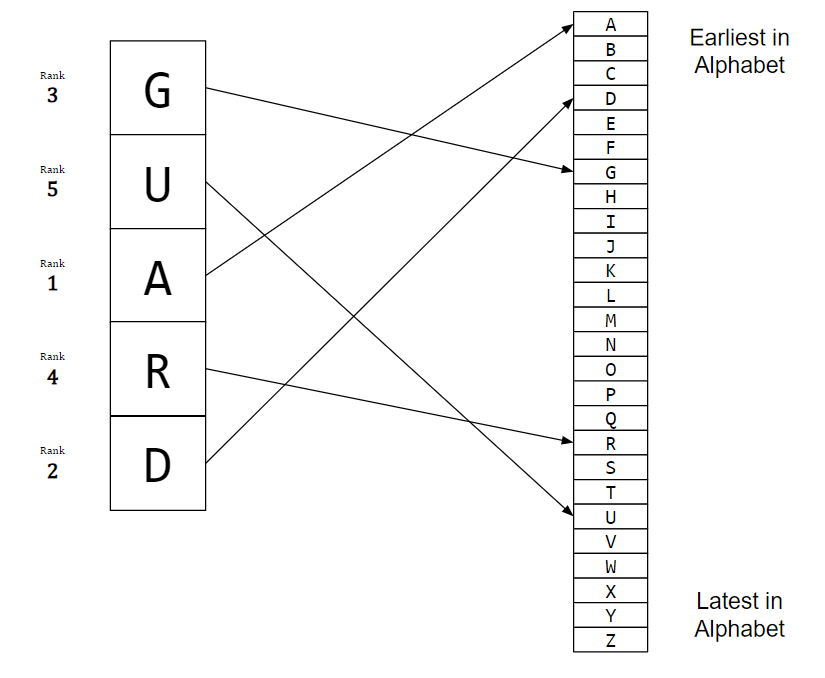
\includegraphics[scale=0.7]{../assets/rank_crypto.png}
    \end{center}
    We note that the alphabetical rankings of the letters of this keyword are 3, 5, 1, 4, 2. We can see this as a \emph{permutation}; that is, 
    \[1 \mapsto 3 \qquad 2 \mapsto 5 \qquad 3 \mapsto 1 \qquad 4 \mapsto 4 \qquad 5 \mapsto 2\]
    \textbf{The idea for encryption is that, for each column $i$, we'll send that column to whatever is mapped by the permutation above.} Going back to the stack of letters we have, we can label each individual column:
    \begin{mdframed}
        \begin{verbatim}
plaintext 
position    1 2 3 4 5
            H I D E T
            H E B A B
            O O N S A
            R E C O M
            I N G F O
            R Y O U Q\end{verbatim}
    \end{mdframed}
    The idea is that 
    \begin{itemize}
        \item we can put all letters under position 1 in the plaintext stack to position \textbf{3} of the ciphertext stack, 
        \item we can put all letters under position 2 in the plaintext stack to position \textbf{5} of the ciphertext stack, 
        \item we can put all letters under position 3 in the plaintext stack to position \textbf{1} of the ciphertext stack, 
        \item we can put all letters under position 4 in the plaintext stack to position \textbf{4} of the ciphertext stack, 
        \item we can put all letters under position 5 in the plaintext stack to position \textbf{2} of the ciphertext stack.
    \end{itemize}
    The process, visually, would look like: 
    \begin{center}
        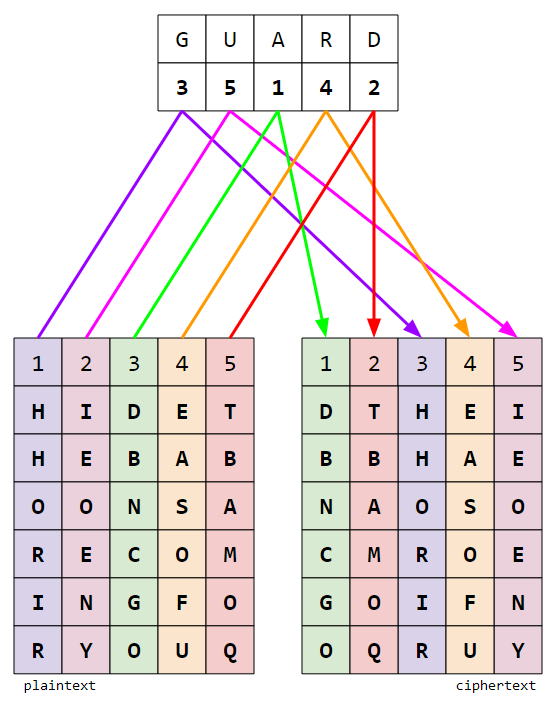
\includegraphics[scale=0.7]{../assets/trans_encrypt.png}
    \end{center}
    Therefore, the ciphertext stack would look like: 
    \begin{mdframed}
        \begin{verbatim}
DTHEI
BBHAE
NAOSO
CMROE
GOIFN
OQRUY\end{verbatim}
    \end{mdframed}
    Undoing the stacking gives us the ciphertext: 
    \begin{mdframed}
        \begin{verbatim}
DTHEIBBHAENAOSOCMROEGOIFNOQRUY\end{verbatim}
    \end{mdframed}
\end{mdframed}
\textbf{Remark:} An easy way to run through the process is to create two ``groups,'' side-by-side. The first group will be the plaintext stack, and the second group will be the ciphertext text. Then, label each column of the first group with the \textbf{alphabetical ranking} of the keyword. Label each column of the second group with \textbf{12345}. Finally, map each column from the first group to the second group based on the label. 
\begin{center}
    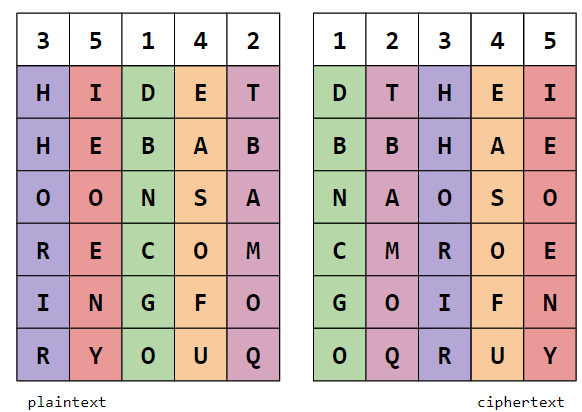
\includegraphics[scale=0.7]{../assets/trans_encrypt2.png}
\end{center} 

Decrypting is merely the inverse of the encryption process.
\begin{mdframed}
    (Example: Decryption.) Consider the above example again. Suppose Alice successfully sends the following ciphertext to Bob:
    \begin{mdframed}
        \begin{verbatim}
DTHEIBBHAENAOSOCMROEGOIFNOQRUY\end{verbatim}
    \end{mdframed}
    Bob knows that the keyword is \code{GUARD}. He can use this keyword to decrypt the message. He can begin by taking the letters of the ciphertext and stacking them into rows of 5, since \code{GUARD} has 5 letters:
    \begin{mdframed}
        \begin{verbatim}
DTHEI
BBHAE
NAOSO
CMROE
GOIFN
OQRUY\end{verbatim}
    \end{mdframed}
    Bob also knows the alphabetical ranking of the letters of \code{GUARD} (which is the same rankings as described above). In particular, the alphabetical ranking is \code{35142}. So, we need to do the following: 
    \begin{itemize}
        \item The letters in position 1 of the ciphertext stack needs to be moved to position \textbf{3},
        \item the letters in position 2 of the ciphertext stack needs to be moved to position \textbf{5},
        \item the letters in position 3 of the ciphertext stack needs to be moved to position \textbf{1},
        \item the letters in position 4 of the ciphertext stack needs to be moved to position \textbf{4},
        \item the letters in position 5 of the ciphertext stack needs to be moved to position \textbf{2}. 
    \end{itemize}
    
    The process, visually, would look like: 
    \begin{center}
        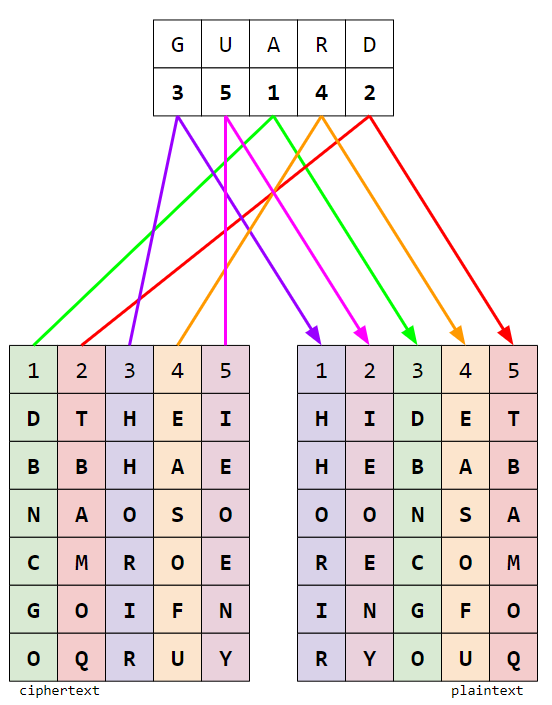
\includegraphics[scale=0.7]{../assets/trans_decrypt.png}
    \end{center}
    Undoing the stacking gives us:
    \begin{mdframed}
        \begin{verbatim}
HIDETHEBABOONSARECOMINGFORYOUQ\end{verbatim}
    \end{mdframed}
    At this point, Bob needs to make an educated guess as to what the encoded message says (recall that we had to encode the message before encrypting it). By removing the \code{Q} and correctly punctuating the message, we get 
    \begin{mdframed}
        \begin{verbatim}
Hide! The baboons are coming for you.\end{verbatim}
    \end{mdframed}
\end{mdframed}
\textbf{Remark:} We can easily decrypt an encrypted word by doing the inverse of what we did above. Create two ``groups,'' side-by-side. The first group will be the ciphertext stack, and the second group will be the plaintext text. Then, label each column of the first group with \textbf{12345}. Label each column of the second group with the \textbf{alphabetical ranking} of the keyword. Finally, map each column from the first group to the second group based on the label. 
\begin{center}
    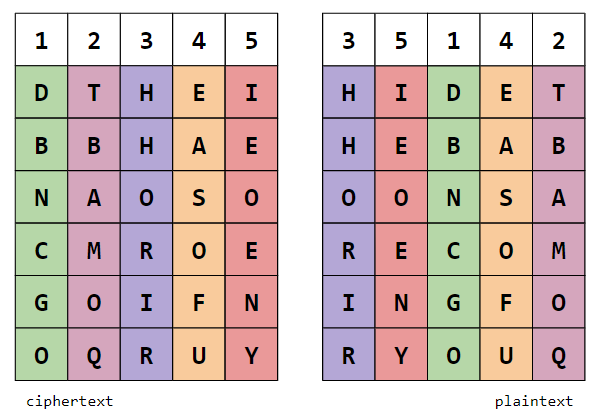
\includegraphics[scale=0.7]{../assets/trans_decrypt2.png}
\end{center} 

\begin{mdframed}[nobreak=true]
    (Exercise: Encryption.) \emph{Encrypt the message \code{There is always hope.} using the keyword \code{CRASH}.}

    \begin{mdframed}
        First, we encode the message so that we can easily encrypt it: 
        \begin{mdframed}
            \begin{verbatim}
THEREISALWAYSHOPE\end{verbatim}
        \end{mdframed}

        Noting that \code{CRASH} has length 5, we break the now encoded message into groups of 5 letters (5-grams):
        \begin{mdframed}
            \begin{verbatim}
THERE
ISALW
AYSHO
PE\end{verbatim}
        \end{mdframed}
        
        Let's now add nonsense letters at the end of the last row so every row has 5 letters: 
        \begin{mdframed}
            \begin{verbatim}
THERE
ISALW
AYSHO
PEABC\end{verbatim}
        \end{mdframed}

        Now, we note the alphabetical ranking of each letter in \code{CRASH}:
        \[C \mapsto 2 \quad R \mapsto 4 \quad A \mapsto 1 \quad S \mapsto 5 \quad H \mapsto 3.\]
        Using the streamlined way discussed above, we have 
        \begin{mdframed}
            \begin{verbatim}
2 4 1 5 3 | 1 2 3 4 5
T H E R E | E T E H R
I S A L W | A I W S L
A Y S H O | S A O Y H
P E A B C | A P C E B\end{verbatim}
        \end{mdframed}
        Unstacking the new rows gives us the ciphertext:
        \begin{mdframed}
            \begin{verbatim}
ETEHRAIWSLSAOYHAPCEB\end{verbatim}
        \end{mdframed}
    \end{mdframed}
\end{mdframed}


\begin{mdframed}[nobreak=true]
    (Exercise: Decryption.) \emph{Decrypt the message \code{ETIHGFREAFRSLAESOXOE} using the keyword \code{CRASH}.}

    \begin{mdframed}
        Begin by grouping the letters into 5-grams, since \code{CRASH} has length 5:
        \begin{mdframed}
            \begin{verbatim}
ETIHG
FREAF
RSLAE
SOXOE\end{verbatim}
        \end{mdframed}
        Recall that the alphabetical ranking of each letter in \code{CRASH} is \code{24153}. Using the streamlined way discussed above, we have 
        \begin{mdframed}
            \begin{verbatim}
1 2 3 4 5    2 4 1 5 3
E T I H G -> T H E G I 
F R E A F -> R A F F E 
R S L A E -> S A R E L 
S O X O E -> O O S E X \end{verbatim}
        \end{mdframed}
        Unstacking the new rows gives us the plaintext:
        \begin{mdframed}
            \begin{verbatim}
THEGIRAFFESARELOOSEX\end{verbatim}
        \end{mdframed}
        Decoding the message gives us: 
        \begin{mdframed}
            \begin{verbatim}
The giraffes are loose.\end{verbatim}
        \end{mdframed}
    \end{mdframed}

\end{mdframed}

\begin{mdframed}
    (Exercise.) Encrypt the message \code{Meet at the trolley station.} using keyword \code{UCSD}.

    \begin{mdframed}
        Encoding, grouping the resulting letters into groups of 4, and adding a nonsense letter gives us: 
        \begin{verbatim}
MEET
ATTH
ETRO
LLEY
STAT
IONX\end{verbatim}
        Noting that the alphabetical ranking of \code{UCSD} is \code{4132}, we can use the streamlined way discussed above to get the encrypted result:
        \begin{mdframed}
            \begin{verbatim}
4 1 3 2    1 2 3 4
M E E T -> E T E M
A T T H -> T H T A
E T R O -> T O R E
L L E Y -> L Y E L
S T A T -> T T A S
I O N X -> O X N I\end{verbatim}
        \end{mdframed}
        Unstacking the result gives us:
        \begin{mdframed}
            \begin{verbatim}
/ETEMTHTATORELYELTTASOXNI\end{verbatim}
        \end{mdframed}
    \end{mdframed}
\end{mdframed}

\begin{mdframed}
    (Exercise.) Alice and Bob share the keyword \code{ZEUS}. Alice uses rectangular tranposition to encrypt the following nonsense message: 
    \begin{verbatim}
MTSQAGXY\end{verbatim}
    What is the corresponding ciphertext? 
    \begin{mdframed}
        Encoding, grouping the resulting letters into groups of 4, and adding a nonsense letter gives us: 
        \begin{mdframed}
            \begin{verbatim}
MTSQ
AGXY\end{verbatim}
        \end{mdframed}
        Noting that the alphabetical ranking of \code{ZEUS} is \code{4132}, we can use the streamlined way discussed above to get the encrypted result:
        \begin{mdframed}
            \begin{verbatim}
4 1 3 2    1 2 3 4
M T S Q -> T Q S M
A G X Y -> G Y X A\end{verbatim}
        \end{mdframed}
        Unstacking the result gives us:
        \begin{mdframed}
            \begin{verbatim}
TQSMGYXA\end{verbatim}
    \end{mdframed}
    \end{mdframed}
\end{mdframed}

\begin{mdframed}
    (Exercise.) The following message was encrypted using rectangular transposition with the keyword \code{SNAKE}. What is the plaintext? 
    \begin{verbatim}
        DSUEMSEDIAJQQDA\end{verbatim}
    
    \begin{mdframed}
        \code{SNAKE} has alphabetical ranking \code{54132}. With this in mind, stacking the letters of the encrypted message into groups of 5 and then running the streamlined process gives us: 
        \begin{mdframed}
\begin{verbatim}
1 2 3 4 5    5 4 1 3 2   
D S U E M -> M E D U S
S E D I A -> A I S D E
J Q Q D A -> A D J Q Q\end{verbatim}
        \end{mdframed}

        Unstacking the result gives us: 
        \begin{mdframed}
\begin{verbatim}
MEDUSAISDEADJQQ\end{verbatim}
        \end{mdframed}
        Decoding gives us: 
        \begin{mdframed}
\begin{verbatim}
Medusa is dead.\end{verbatim}
        \end{mdframed}
    \end{mdframed}
\end{mdframed}


\subsection{Masonic Cipher}
The masonic cipher (also known as the \emph{pigpen cipher} or \emph{tic-tac-toe cipher}) is a simple substitution cipher that replaces individual letters with certain geometric shapes.

\bigskip 

For example, consider the following diagram, which represents a Masonic cipher for the English letters:
\begin{center}
    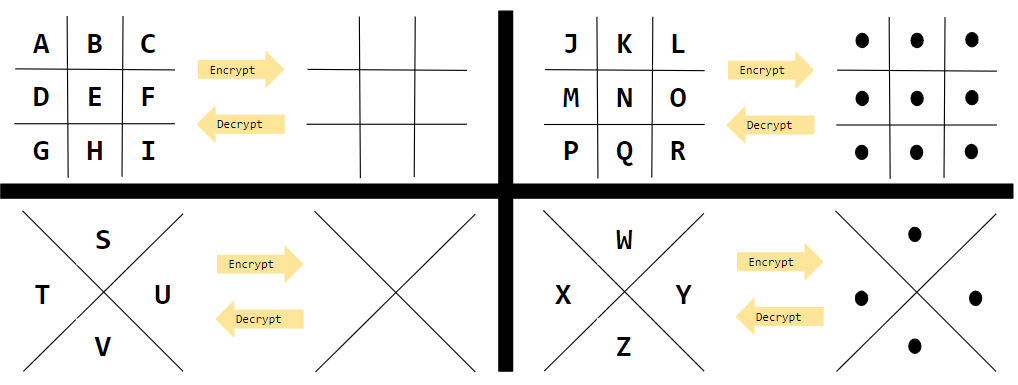
\includegraphics[scale=0.75]{../assets/masonic_ex1.png}
\end{center}
The idea is that we can replace a letter (e.g., \code{A}) with a corresponding geometric shape (e.g., the backwards \code{L} represented by the top-left part of the grid.) 

\bigskip 

Some other examples based on the above cipher are shown below:
\begin{center}
    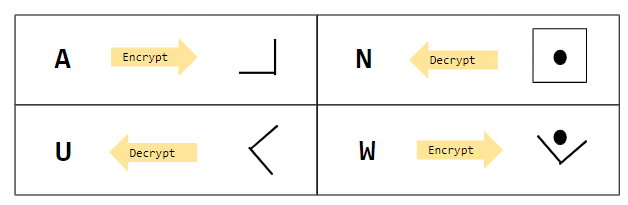
\includegraphics[scale=0.9]{../assets/masonic_ex2.png}
\end{center}
Note that there is \emph{no key} associated with this cipher. There is only a decryption function (which is just mapping the geometric shape back to the letter). Therefore, the adversary, who knows that a message was encrypted using a masonic cipher, can recover the plaintext easily. 


\subsection{Caesar Cipher}
The Caesar cipher, also known as a \emph{shift cipher}, is a simple substitution cipher that \emph{shifts} a letter by some amount $n$. Hence, the key for this cipher is an integer $n$. The idea is that we initially assign each letter an integer, perhaps by their alphabetical ranking (e.g., $A$ is 0, $B$ is 1, and so on.) If we want to shift the letters by some number, we can just ``move'' the letters by that amount. If a letter gets a new integer that's greater than 25, we can ``wrap'' the letter back.  

\bigskip 

Consider the following diagram, which shows the correspondence between the plaintext alphabet and the ciphertext alphabet.
\begin{center}
    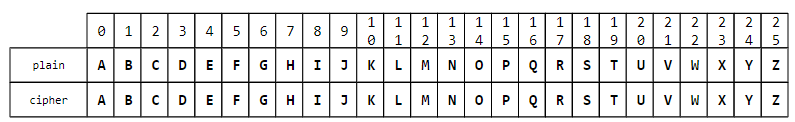
\includegraphics[scale=0.75]{../assets/ceasar_1.png}
\end{center}
In this particular diagram, when we apply a shift, we apply the shift to the \emph{plain} row. By doing this, we can translate whatever plaintext we have to ciphertext. 

\begin{mdframed}
    (Example.) If we shift each letter by 3 (i.e., $n = 3$), we have 
    \begin{center}
        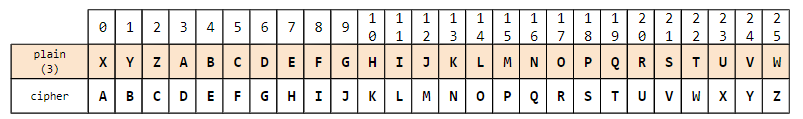
\includegraphics[scale=0.7]{../assets/ceasar_2.png}
    \end{center}
    Notice how $A$ now corresponds to 3. Recall that $A$'s original position was 0; if we shift each letter by 3, we essentially add 3 to $A$'s original position to get the new position 
    \[0 + 3 = 3.\]
    The same idea applies to any other letter. One key thing to notice is how $X$, $Y$, and $Z$ were \emph{wrapped back} to the beginning. In any case, let's see how translation would work in this case: 
    \begin{itemize}
        \item To convert a letter from plaintext to ciphertext, look for the letter in the(shifted) plaintext row and then look at the corresponding ciphertext column. For example, $R$ in plaintext would become $U$ in ciphertext. 
        \item To convert a letter from ciphertext to plaintext, look for the letter in the ciphertext row and then look at the corresponding (shifted) plaintext column. For example, $U$ in ciphertext becomes $R$ in plaintext. 
    \end{itemize}
\end{mdframed}

\begin{mdframed}
    (Example.) If we shift each letter by -2 (i.e., $n = -2$), we have 
    \begin{center}
        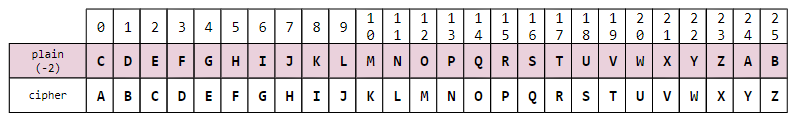
\includegraphics[scale=0.7]{../assets/ceasar_3.png}
    \end{center}
\end{mdframed}

As with rectangular tranposition, we should encode the message by removing any non-alphabetic characters and capitalizing everything. 

\begin{mdframed}
    (Exercise.) 
    \begin{itemize}
        \item \emph{Using a shift of 3, encrypt the message \code{Meet at La Jolla Shores.}}
        \begin{mdframed}
            Encoding the message gives us \code{MEETATLAJOLLASHORES}. Then, we can use the example above (with the shift of 3) to give us the proper correspondence.
            \begin{verbatim}
    plain       M E E T A T L A J O L L A S H O R E S
    cipher      P H H W D W O D M R O O D V K R U H V\end{verbatim}
            This gives us \code{PHHWDWODMROODVKRUHV}.
        \end{mdframed}
        \item \emph{Using a shift of 3, decrypt the message \code{PHHWDWVXQJRGODZQ}}
        \begin{mdframed}
            Using the example above (with the shift of 3), we have
            \begin{verbatim}
    cipher      P H H W D W V X Q J R G O D Z Q
    plain       M E E T A T S U N G O D L A W N\end{verbatim}
            Decoding this gives us \code{Meet at Sun God Lawn.}
        \end{mdframed}
    \end{itemize}
\end{mdframed}

\begin{mdframed}
    (Exercise.) \emph{You are Eve. You have just intercepted the following message that Alice was trying to send to Bob: \code{Q TQDM IB QPWCAM}. You know that Alice used a Caesar cipher, but she didn't remove spaces before encrypting: she left the spaces in her original message as-is. What is the original message?}
    
    \begin{mdframed}
        \code{Q} itself could be a word; specifically, it could either be \code{A} or \code{I}. We can try to figure out what the message by guessing which word the first word could be. 
        \begin{itemize}
            \item If \code{Q} maps to \code{A}, then we have 
            \begin{center}
                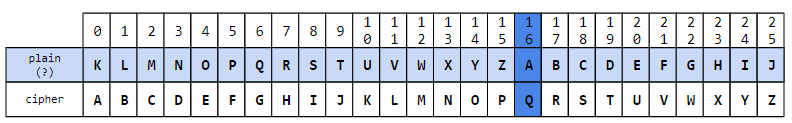
\includegraphics[scale=0.6]{../assets/ceasar_4.png}
            \end{center}
            Partially decrypting the ciphertext gives us \code{A DANW}, but \code{DANW} is meaningless. Therefore, it cannot be \code{A}. 

            \item If \code{Q} maps to \code{I}, then we have
            \begin{center}
                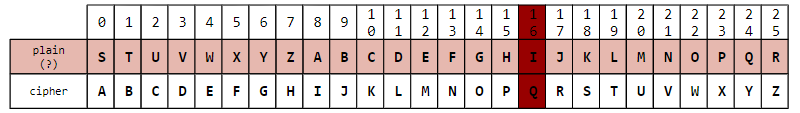
\includegraphics[scale=0.6]{../assets/ceasar_5.png}
            \end{center}
            Decrypting this gives us: 
            \begin{verbatim}
                I LIVE AT IHOUSE\end{verbatim}
        \end{itemize}
        Therefore, the message is \code{I LIVE AT IHOUSE}. The shift was 8.
    \end{mdframed}
\end{mdframed}


\begin{mdframed}
    (Exercise.) Alice encrypts the following message using a Caesar cipher with a shift of 1. 
    \begin{verbatim}
Zeus is hiding in a cave \end{verbatim}
    What is the corresponding ciphertext? 
    \begin{mdframed}
        \begin{verbatim}
plain       ZEUSISHIDINGINACAVE
cipher      AFVTJTIJEJOHJOBDBWF\end{verbatim}
        Essentially, we just move all letters forward by 1.
    \end{mdframed}
\end{mdframed}

\end{document}